\documentclass{article}
\usepackage{amsmath}
\usepackage{tikz}
\usetikzlibrary{positioning}

\begin{document}

\begin{figure}[h]
    \centering
    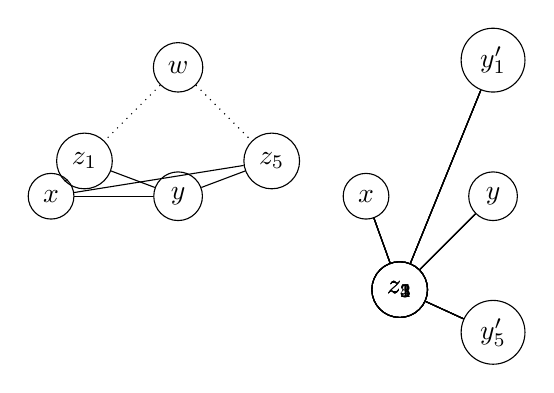
\begin{tikzpicture}[node distance=1cm, auto]
        % Define nodes
        \node (x) [circle, draw] {$x$};
        \node (y) [circle, draw, right=of x] {$y$};
        \node (w) [circle, draw, above=of y] {$w$};
        \node (z1) [circle, draw, below left=of w] {$z_1$};
        \node (z5) [circle, draw, below right=of w] {$z_5$};
        
        % Draw edges
        \draw (x) -- (y);
        \draw (x) -- (z1);
        \draw (x) -- (z5);
        \draw (y) -- (z1);
        \draw (y) -- (z5);
        \draw[dotted] (w) -- (z1);
        \draw[dotted] (w) -- (z5);
        
        % Second part of the figure
        \begin{scope}[xshift=4cm]
            \node (x') [circle, draw] {$x$};
            \node (y') [circle, draw, right=of x'] {$y$};
            \node (y1') [circle, draw, above=of y'] {$y'_1$};
            \node (y5') [circle, draw, below=of y'] {$y'_5$};
            
            \foreach \i in {1,...,5} {
                \node (z\i) [circle, draw, below left=of y'] {$z_\i$};
                \draw (x') -- (z\i);
                \draw (y') -- (z\i);
            }
            
            \foreach \i in {1,...,5} {
                \draw (z\i) -- (y1');
                \draw (z\i) -- (y5');
            }
        \end{scope}
    \end{tikzpicture}
    \caption{Left: The case \( S \nsubseteq N[x] \cup N[y] \) and \( |Z| \geq 5 \) in the proof of the second statement in Claim~\ref{clm2}. Right: The proof of Claim~\ref{clm3}, where we suppose, to the contrary, that there exists \( x_i \) such that \( |N(x_i) \cap Y| \geq 5 \).}
    \label{fig:claim_diagrams}
\end{figure}

\end{document}